% Provenance (never printed): see sources/outline_sources.md (Year 2: monsoons; El Niño--Southern
% Oscillation; the North Atlantic Oscillation; ocean--atmosphere coupling). Definitions after the
% IPCC AR6 glossary, the NOAA CPC ENSO FAQ and NAO pages, the NWS glossary and the IMD monsoon
% FAQ; indices from the CPC data files (data/derived/bachelor-2-{oni,oni-table,roni,nino34,nao});
% figures from figdata/bachelor-2/climvar.py; values of the examples, exercises and problem
% computed in the Book 4 scratch calculator calc/ch23.py.
\chapter{Variabilité climatique}\label{ch:b2:climate-variability}

En septembre 2026, la température de surface de la mer dans le Pacifique équatorial central
moyennait \qty{29.27}{\celsius}, alors que la valeur habituelle de septembre est de \qty{26.71}{\celsius}~; plus à l'est, des
parties de l'océan étaient de plus de \qty{4}{\celsius} plus chaudes que d'ordinaire, et les prévisionnistes donnaient
plus de quatre chances sur cinq que l'événement dépasse, d'ici la fin de l'année,
tous les El~Niño depuis 1950. Les épisodes records précédents, en 1982, 1997 et 2015,
ont blanchi et tué des coraux, incendié des forêts tropicales et apporté des canicules~;
la pêche d'anchois du Pérou chute fortement lorsque cette eau chaude persiste. L'océan et
l'atmosphère du Pacifique tropical avaient basculé, comme ils le font tous les quelques ans,
et ce basculement dépassait largement le Pacifique. Ce chapitre décrit ces basculements du climat,
les \omterm{def:b2:climate-variability:monsoon}{moussons}, El~Niño et La~Niña, l'\omterm{def:b2:climate-variability:nao}{oscillation nord-atlantique}, et ce qui fait de l'océan leur mémoire.
% ledger: data:b4-nino34, cpc:edd-2026-10, thirumalai24:bjerknes, cheung26:peru

\begin{recall}
\textbf{Des volumes scolaires}~: le temps et le climat~; l'anomalie de température~; la couche de mélange,
la thermocline et les remontées d'eau~; la rétroaction climatique. \textbf{Du volume de première année}~: les
cellules de Hadley, les alizés, la zone de convergence intertropicale et sa migration saisonnière,
la circulation de Walker, les remontées côtières d'eau froide. \textbf{Du \cref{ch:b2:weather-systems}}~: le
courant-jet, les \omterm{def:b2:weather-systems:rossby}{ondes de Rossby}, les cyclones extratropicaux et le blocage. \textbf{Des volumes de physique}~:
la capacité thermique et le premier principe de la thermodynamique.
\end{recall}

\section{Variabilité et ses mesures}\label{sec:b2:climate-variability:measures}

Le temps change d'un jour à l'autre~; le climat, qui est la statistique du temps, change lui aussi,
d'une saison ou d'une année à l'autre, même lorsque rien ne change hors du système climatique.
Une partie de cette variabilité est du bruit, mais une grande part s'organise en quelques
configurations récurrentes, dotées de leur géographie et de leurs échelles de temps propres.

\begin{definition}[Mode de variabilité climatique~; indice climatique~; climatologie]\label{def:b2:climate-variability:modes}
Un \emph{mode de variabilité climatique}\index{mode de variabilité climatique} est un motif récurrent
de la variabilité naturelle du système climatique, doté de sa propre structure spatiale, de sa saisonnalité et de ses échelles de temps,
né de la dynamique de l'atmosphère ou du couplage entre l'océan et l'atmosphère.
Un \emph{indice climatique}\index{indice climatique} est une série temporelle construite à partir de variables climatiques,
qui résume l'état d'un tel motif, par exemple la différence de pression au niveau de la mer entre l'Islande et les Açores.
La \emph{climatologie}\index{climatologie} d'une variable est sa moyenne sur une période de référence,
calculée pour chaque mois du calendrier ou chaque saison~; la période de référence standard dure 30 ans,
soit actuellement 1991--2020.
\end{definition}
% ledger: ipccgl:modes, ipccgl:index, wmo:normal-30yr

De nombreux modes sont entretenus par des processus internes au système climatique~: ils font partie de sa
variabilité interne. Comme ils reviennent avec leurs propres échelles de temps, ils sont une source de
prévisibilité au-delà de la portée des prévisions météorologiques, de quelques semaines à quelques décennies. Les indices
les rendent mesurables. Un indice se calcule à partir d'anomalies, comme dans les volumes scolaires, puis il est
lissé.
% ledger: ipccgl:modes

\begin{method}[Des observations à un indice]\label{met:b2:climate-variability:index}
\begin{enumerate}
\item Calculer la \omterm{def:b2:climate-variability:modes}{climatologie}~: la moyenne de la variable pour chaque mois du calendrier sur la
période de référence.
\item La soustraire~: l'anomalie de chaque mois est sa valeur moins la \omterm{def:b2:climate-variability:modes}{climatologie} de ce mois.
Le cycle saisonnier disparaît~; il ne reste que la variabilité.
\item Lisser les anomalies par une moyenne glissante, c'est-à-dire la moyenne de $n$ valeurs consécutives centrée sur
chaque mois, pour éliminer les fluctuations plus courtes que le motif étudié.
\item Si l'indice doit être comparé à d'autres, le diviser par son écart type~: l'indice est alors
normalisé, exprimé en nombre d'écarts types.
\end{enumerate}
\end{method}

\begin{example}[Une anomalie]\label{ex:b2:climate-variability:anomaly}
La température de surface moyenne de la mer dans le Pacifique équatorial central, entre \ang{5}~N et
\ang{5}~S, \ang{170}~O et \ang{120}~O, était de \qty{29.27}{\celsius} en septembre 2026. Sa \omterm{def:b2:climate-variability:modes}{climatologie} de septembre
est de \qty{26.71}{\celsius}, donc l'anomalie valait $29.27 - 26.71 = \qty{2.56}{\celsius}$.
En septembre 1997, le même océan était à \qty{28.79}{\celsius} contre \qty{26.73}{\celsius}, soit une
anomalie de \qty{2.06}{\celsius}. Les deux \omterm{def:b2:climate-variability:modes}{climatologies} diffèrent légèrement parce que la période de
référence est déplacée tous les cinq ans~: l'océan lui-même s'est réchauffé.
% ledger: data:b4-nino34, cpc:oni-def
\end{example}

\section{Moussons}\label{sec:b2:climate-variability:monsoons}

\begin{definition}[Mousson]\label{def:b2:climate-variability:monsoon}
Une \emph{mousson}\index{mousson} est un vent d'origine thermique, né du contraste de chauffage entre une masse
continentale et l'océan voisin, qui change de sens avec les saisons, ainsi que
l'inversion saisonnière des pluies qu'il apporte.
\end{definition}
% ledger: nws4:monsoon, ipccgl:monsoon

Sur terre, la chaleur du soleil d'été reste dans une fine couche près de la surface, tandis que la mer la répartit
sur sa couche de mélange, de plusieurs dizaines de mètres d'épaisseur, et se réchauffe bien moins. L'air au-dessus
des continents se réchauffe davantage, sa pression au sol baisse, et l'air humide venu de la mer s'élève, se refroidit
et pleut~; en altitude, l'air repart vers la mer. En hiver, la terre est la surface la plus froide et la circulation
s'inverse. Pris ensemble, les \omterm{def:b2:climate-variability:monsoon}{moussons} de la planète forment un seul motif global qui domine le cycle annuel des
pluies tropicales et subtropicales~; leur domaine est défini comme les régions où la pluie moyenne de l'été local
dépasse celle de l'hiver de plus de \qty{2.5}{mm} par jour.
% ledger: nws4:monsoon, ipccgl:monsoon

\begin{omfigure}
\centering
\begin{tikzpicture}[font=\scriptsize, >=Stealth]
\foreach \col/\title in {0/{a\enspace été}, 7.2/{b\enspace hiver}} {
  \begin{scope}[shift={(\col,0)}]
  \node[anchor=south west] at (0,3.0) {\textbf{\title}};
  \fill[ocBlue!18] (0,0) rectangle (3,0.35);
  \fill[brown!35] (3,0) -- (6.4,0) -- (6.4,0.5) -- (3,0.35) -- cycle;
  \node at (1.5,0.17) {mer};
  \node at (4.7,0.2) {terre};
  \end{scope}
}
% summer: low over the land, inflow from the sea, rising air and rain
\node[font=\small\bfseries, ocBlue] at (0.45,0.62) {H};
\node[font=\small\bfseries, ocRed] at (4.8,0.78) {L};
\node[ocRed, anchor=west] at (5.35,0.78) {chaud};
\draw[->, thick] (1.0,0.98) -- (4.2,1.02);
\node at (2.4,0.66) {air humide venu de la mer};
\draw[->, thick] (4.8,1.15) -- (4.8,2.55);
\draw[->, thick] (4.45,2.8) -- (1.75,2.8);
\draw[->, thick] (1.4,2.6) -- (1.4,1.25);
\fill[black!15, draw=black!40] (4.0,1.9) .. controls (4.0,2.55) and (5.6,2.55) .. (5.6,1.9) -- cycle;
\foreach \x in {4.25,4.5,5.1,5.35} {\draw[ocBlue, dashed] (\x,1.85) -- (\x-0.1,1.2);}
\node[anchor=west] at (5.65,2.1) {pluie};
% winter: high over the land, dry outflow to the sea
\begin{scope}[shift={(7.2,0)}]
\node[font=\small\bfseries, ocRed] at (0.45,0.62) {L};
\node[font=\small\bfseries, ocBlue] at (4.8,0.78) {H};
\node[ocBlue, anchor=west] at (5.35,0.78) {froid};
\draw[->, thick] (4.2,1.02) -- (1.0,0.98);
\node at (2.4,0.66) {air sec venu de la terre};
\draw[->, thick] (1.4,1.25) -- (1.4,2.6);
\draw[->, thick] (1.75,2.8) -- (4.45,2.8);
\draw[->, thick] (4.8,2.55) -- (4.8,1.15);
\end{scope}
\end{tikzpicture}
\par\smallskip{\small La \omterm{def:b2:climate-variability:monsoon}{mousson} vue comme une circulation terre--mer (coupe schématique, non à l'échelle)~: en été, la terre est la surface la plus chaude,
avec une basse pression au sol, un afflux d'air humide venu de la mer, un air ascendant et des pluies~; en hiver, la circulation s'inverse et le vent
venu de la terre est sec.}
\end{omfigure}
% ledger: nws4:monsoon, imd:heat-low

La \omterm{def:b2:climate-variability:monsoon}{mousson} de l'Asie du Sud et du Sud-Est commence fin mai ou début juin, progresse vers le nord-est
et se termine fin septembre ou début octobre. Auparavant, les terres qui bordent la mer d'Arabie se réchauffent~:
en juin, la surface envoie environ \qty{160}{W/m^2} de chaleur dans l'air du nord-ouest aride de l'Inde,
du Pakistan et du Moyen-Orient, où se forme une basse thermique peu épaisse, qui ne s'élève qu'à environ
\qty{1.5}{km}, avec peu de pluie~; une basse thermique faible, comme lors de la sécheresse de 1987,
signifie une faible aspiration de l'air humide de l'océan. De celle-ci part une dépression allongée,
le talweg de \omterm{def:b2:climate-variability:monsoon}{mousson}, qui s'étend jusqu'à la tête du golfe du Bengale~; ses oscillations nord--sud
amènent les phases actives et les pauses de la saison. Sur l'ensemble de l'Inde, la pluie de juin à septembre
moyenne \qty{88}{cm}, avec un écart type de \qty{9}{cm}, soit environ \qty{10}{\percent}~: une saison située à moins de
\qty{10}{\percent} de la moyenne de longue période est dite normale. Sur la côte du Kerala, où le service
météorologique national annonce le début de la \omterm{def:b2:climate-variability:monsoon}{mousson} d'après les pluies de quatorze stations, les vents et le
rayonnement infrarouge sortant mesuré par satellite, la pluie moyenne est de \qty{556}{mm} en juin et
\qty{659}{mm} en juillet.
% ledger: ipccgl:monsoon, imd:heat-low, imd:lpa, imd:onset

La \omterm{def:b2:climate-variability:monsoon}{mousson} d'Afrique de l'Ouest apporte des vents humides de sud-ouest venus du golfe de Guinée, qui progressent
vers le nord de mai à septembre~; ses pluies culminent vers \ang{12}~N fin août et en septembre,
puis se retirent à partir d'octobre.
% ledger: ipccgl:monsoon

Une \omterm{def:b2:climate-variability:monsoon}{mousson} est régulière dans son calendrier, irrégulière dans sa quantité, et les oscillations annuelles du
Pacifique tropical en sont parmi les causes. Les années El~Niño laissent souvent l'Inde en manque de pluie~: les
sécheresses de 1904, 1972 et 1987 sont venues avec El~Niño. Le lien n'est pas certain~: en 1997, un fort El~Niño
a coïncidé avec une phase positive du dipôle de l'océan Indien, un mode évoqué plus loin, et l'Inde a eu une
\omterm{def:b2:climate-variability:monsoon}{mousson} proche de la normale.
% ledger: narang24:enso-monsoon, ipccgl:other-modes

\section{El~Niño et oscillation australe}\label{sec:b2:climate-variability:enso}

Le volume de première année a décrit la circulation de Walker~: l'air monte au-dessus du Pacifique occidental
chaud, s'écoule vers l'est en altitude, descend au-dessus du Pacifique oriental froid et revient vers l'ouest
avec les alizés. Dans l'océan, les alizés accumulent l'eau chaude à l'ouest, où la thermocline est profonde,
et font remonter l'eau froide le long de l'équateur, à l'est, où elle est peu profonde.
Cet état n'est pas figé.

\begin{definition}[El Niño--Oscillation australe~; El~Niño~; La~Niña~; oscillation australe]\label{def:b2:climate-variability:enso}
L'\emph{El Niño--Oscillation australe}\index{El Niño--Oscillation australe} (ENSO) est le mode couplé océan--atmosphère
du Pacifique tropical~: des variations cohérentes d'une année à l'autre de la température de surface de la mer,
des précipitations convectives, de la pression de surface et de la circulation le long
du Pacifique équatorial, avec des échelles de temps privilégiées de deux à environ sept ans.
\emph{El Niño}\index{El Niño} est sa phase chaude, un réchauffement de la surface de la mer du Pacifique
équatorial central et centre-est~; \emph{La Niña}\index{La Niña} est sa phase froide, un refroidissement
de cette même région. L'\emph{oscillation australe}\index{oscillation australe} est sa composante atmosphérique,
un balancement de la pression de surface entre l'ouest et l'est du Pacifique tropical~: pendant El~Niño,
la pression est supérieure à la moyenne sur l'Indonésie et le Pacifique occidental et inférieure
sur le Pacifique oriental, et l'inverse pendant La~Niña.
\end{definition}
% ledger: cpc:enso-faq, cpc:enso-faq-so, ipccgl:enso

Pendant El~Niño, les alizés d'est faiblissent le long de l'équateur, et à l'ouest les vents de basse altitude peuvent
même souffler d'ouest~; l'eau chaude de l'ouest s'étend vers l'est, et la convection profonde ainsi que sa pluie la suivent,
ce qui laisse l'Indonésie et le nord de l'Australie plus secs.
La surface de la mer du Pacifique centre-est est en général plus chaude que la moyenne de \qtyrange{1.5}{2.5}{\celsius},
et la thermocline y est à \qtyrange{150}{175}{m}, plus profonde que d'habitude.
Pendant La~Niña, les alizés se renforcent sur tout le bassin,
la surface de la mer est plus froide que la moyenne de \qtyrange{1}{2}{\celsius}, et la thermocline à l'est remonte à
\qtyrange{50}{100}{m}. La circulation de Walker s'affaiblit pendant El~Niño et se renforce pendant La~Niña. Les épisodes
reviennent en général tous les trois à cinq ans, à des intervalles allant de deux à sept ans~; un El~Niño dure en général
neuf à douze mois, une La~Niña un à trois ans. Les deux tendent à se développer entre mars et juin, à culminer entre
décembre et avril et à s'affaiblir entre mai et juillet~; leurs effets sont les plus forts de décembre à avril, lorsque la
mer équatoriale est la plus chaude.
% ledger: cpc:enso-faq-features, cpc:enso-faq-timing

\begin{omfigure}
\centering
\begin{tikzpicture}[font=\scriptsize, >=Stealth, x=1cm, y=0.8cm]
\foreach \row/\title/\tw/\te/\rx/\cwidth in {
    0/{a\enspace neutre}/1.15/0.35/1.6/1.0,
    -4.6/{b\enspace El Niño}/0.95/0.85/5.6/1.4,
    -9.2/{c\enspace La Niña}/1.3/0.18/1.0/0.8} {
  \begin{scope}[shift={(0,\row)}]
  \node[anchor=south west] at (0,2.55) {\textbf{\title}};
  % ocean: warm layer above the thermocline
  \fill[ocBlue!20] (0,-1.5) rectangle (11,0);
  \fill[omWarm!25] (0,0) -- (0,-\tw) .. controls (4,-\tw) and (7,-\te) .. (11,-\te) -- (11,0) -- cycle;
  \draw[thick, ocBlue!70!black] (0,-\tw) .. controls (4,-\tw) and (7,-\te) .. (11,-\te);
  \draw (0,0) -- (11,0);
  % convection and Walker cell
  \fill[black!15, draw=black!40] ({\rx-\cwidth/2},0.5) .. controls ({\rx-\cwidth/2},2.1) and ({\rx+\cwidth/2},2.1) .. ({\rx+\cwidth/2},0.5) -- cycle;
  \draw[->, thick] (\rx,0.55) -- (\rx,2.15);
  \draw[->, thick] ({\rx+0.4},2.3) -- (9.6,2.3);
  \draw[->, thick] (10.0,2.1) -- (10.0,0.5);
  \draw[->, thick] (9.6,0.3) -- ({\rx+0.7},0.3);
  \end{scope}
}
  \node[anchor=west] at (2.3,1.4) {air ascendant, pluie};
  \node[anchor=east] at (9.9,1.4) {air subsident};
  \node at (6.0,0.55) {alizés};
\node[anchor=west, ocBlue!70!black] at (7.6,-0.95) {thermocline};
  \node[anchor=east] at (4.8,-4.6+1.4) {la pluie migre vers l'est};
  \node at (8.2,-4.6+0.55) {alizés faibles};
  \node at (6.0,-9.2+0.55) {alizés forts};
  \node[ocBlue!70!black, align=center] at (9.6,-9.2-0.8) {eau froide\\près de la surface};
  \node[anchor=north west] at (0,-9.2-1.55) {ouest (Indonésie)};
  \node[anchor=north east] at (11,-9.2-1.55) {est (Amérique du Sud)};
\end{tikzpicture}
\par\smallskip{\small Le Pacifique équatorial le long de l'équateur dans les trois phases de l'ENSO
(schématique, non à l'échelle)~: la circulation de Walker en haut, la couche superficielle chaude et la thermocline en dessous.
En El~Niño, les alizés faiblissent, l'eau chaude et la pluie s'étendent vers l'est et la thermocline à l'est
s'approfondit jusqu'à \qtyrange{150}{175}{m}~; pendant La~Niña, les alizés se renforcent et la thermocline à l'est
remonte à \qtyrange{50}{100}{m}.}
\end{omfigure}
% ledger: cpc:enso-faq-features, climategov:walker

Les noms viennent de siècles et de sciences différents. Les pêcheurs de la côte sud-américaine remarquèrent un
réchauffement de leurs eaux côtières vers Noël, qui perturbait la pêche,
et l'appelèrent El~Niño, le petit garçon. Sir Gilbert Walker découvrit l'\omterm{def:b2:climate-variability:enso}{oscillation australe} dans l'atmosphère,
sans la relier à l'océan. Ce n'est qu'à la fin des années 1960 que Jacob Bjerknes
et d'autres comprirent que les deux étaient un seul phénomène. Les termes La~Niña et neutre s'imposèrent dans les années 1980.
% ledger: climategov:enso-history, ipccgl:enso

\begin{history}[Le petit garçon des pêcheurs]
\begin{minipage}[t]{0.54\linewidth}\vspace{0pt}
Au large de la côte sèche du Pérou, l'eau froide que les vents remontent le long du rivage est riche en nutriments
et alimente une pêcherie productive. Ses pêcheurs connaissaient un réchauffement qui survenait vers Noël, quand le poisson
devenait rare, et lui donnèrent le nom d'enfant de la saison. La pêche d'anchois du Pérou suit encore l'ENSO~:
dans une étude récente, de longues anomalies de température élevées ont rendu une pêche extrêmement faible plus de neuf fois
plus probable, avec une baisse médiane de la pêche d'environ \qty{60}{\percent}~; le fort El~Niño de 1997--1998 ressort
nettement dans la série.
\end{minipage}\hfill
\begin{minipage}[t]{0.42\linewidth}\vspace{0pt}
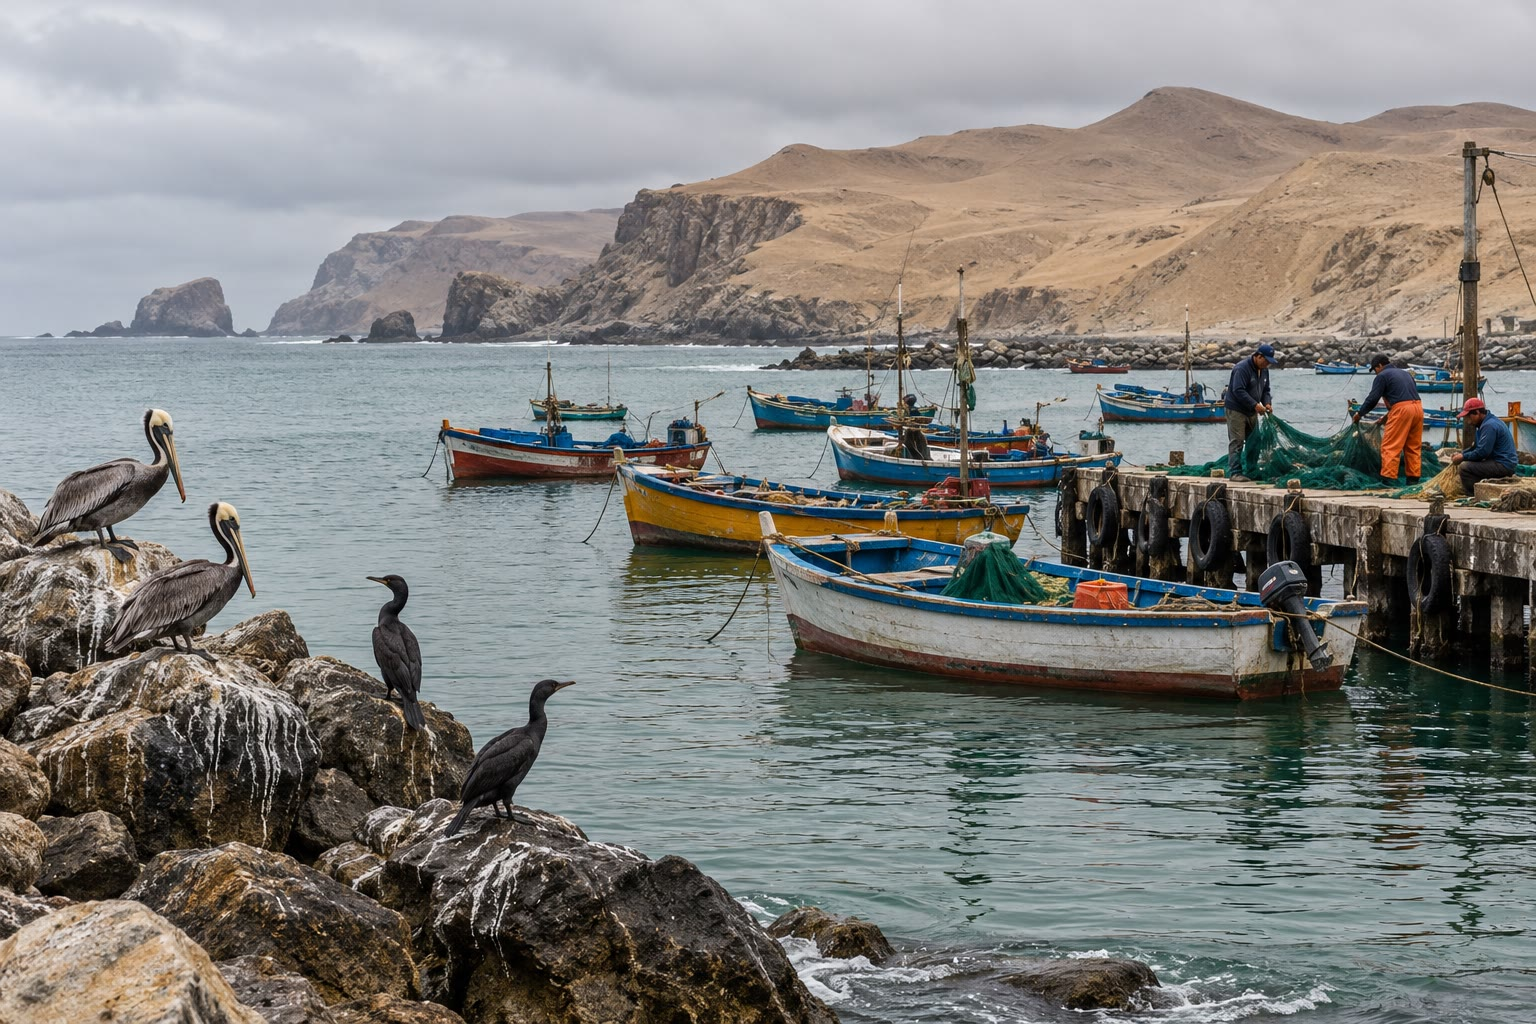
\includegraphics[width=\linewidth]{images/book4/ai/b2-fishing-harbour.jpg}

{\scriptsize Bateaux de pêche dans le port d'une côte désertique où remontent des eaux froides
(Illustration générée par IA.)}
\end{minipage}
% ledger: climategov:enso-history, cheung26:peru, stewart:upwelling
\end{history}

Pourquoi le système oscille-t-il~? Parce que l'océan et l'atmosphère du Pacifique équatorial
renforcent mutuellement leurs anomalies.

\begin{definition}[Rétroaction de Bjerknes]\label{def:b2:climate-variability:bjerknes}
La \emph{rétroaction de Bjerknes}\index{rétroaction de Bjerknes} est la rétroaction positive entre la température
de surface de la mer, les vents et les courants océaniques du Pacifique équatorial~: un réchauffement de l'est affaiblit
le contraste est--ouest de température et de pression, donc les alizés~; des alizés plus faibles laissent l'eau chaude
de l'ouest s'étendre vers l'est et remonter moins d'eau froide à l'est, ce qui réchauffe encore l'est.
La même boucle amplifie un refroidissement.
\end{definition}
% ledger: thirumalai24:bjerknes, cpc:enso-faq-timing

\begin{omfigure}
\centering
\begin{tikzpicture}[font=\small, >=Stealth, box/.style={draw, rounded corners=2pt, fill=omDef!8,
  align=center, text width=4.3cm, minimum height=1.05cm, inner sep=3pt}]
\node[box] (a) at (0,2) {Pacifique équatorial oriental\\plus chaud que d'habitude};
\node[box] (b) at (6.2,2) {contraste est--ouest moindre\\de température et de pression};
\node[box] (c) at (6.2,0) {alizés plus faibles};
\node[box] (d) at (0,0) {l'eau chaude s'étend vers l'est,\\remonte moins d'eau froide};
\draw[->, very thick, ocRed] (a) -- (b);
\draw[->, very thick, ocRed] (b) -- (c);
\draw[->, very thick, ocRed] (c) -- (d);
\draw[->, very thick, ocRed] (d) -- (a);
\node[ocRed, font=\bfseries] at (3.1,1) {$+$};
\end{tikzpicture}
\par\smallskip{\small La \omterm{def:b2:climate-variability:bjerknes}{rétroaction de Bjerknes}, dessinée pour un réchauffement~; en inversant toutes les flèches, la
même boucle approfondit un refroidissement. Une boucle positive de ce type amplifie une petite perturbation.}
\end{omfigure}
% ledger: thirumalai24:bjerknes

Une rétroaction positive explique comment une anomalie croît, et non comment elle commence ou s'achève. Selon une
lecture actuelle, un El~Niño commence lorsque des fluctuations aléatoires des alizés affaiblissent les courants
équatoriaux qui retiennent l'eau chaude à l'ouest~;
la réserve d'eau chaude s'étend vers l'est, la convection
la suit, la \omterm{def:b2:climate-variability:bjerknes}{rétroaction de Bjerknes} prend le relais et l'événement grandit. Les événements La~Niña, selon cette
même lecture, sont déclenchés par un El~Niño précédent. Les modèles les plus simples qui font osciller le système,
dont l'oscillateur de recharge, couplent deux grandeurs~: l'anomalie de température de surface de la mer du Pacifique
central et le volume d'eau chaude stocké dans la couche supérieure de l'océan le long de l'équateur. L'anomalie de
température vide ou remplit ce stock par les vents qu'elle engendre, et le stock, par la profondeur de la thermocline,
prépare la phase suivante. \Cref{exo:b2:climate-variability:10} résout un tel couple d'équations.
% ledger: thirumalai24:bjerknes, stuecker25:ro

Pour suivre l'ENSO, les centres de surveillance utilisent des indices.

\begin{definition}[Indice Niño-3.4~; indice océanique Niño]\label{def:b2:climate-variability:oni}
L'\emph{indice Niño-3.4}\index{indice Niño-3.4} est l'anomalie mensuelle de la température de surface de la mer,
moyennée sur la région \ang{5}~N--\ang{5}~S, \ang{170}~O--\ang{120}~O, par rapport à la \omterm{def:b2:climate-variability:modes}{climatologie}
d'une période de base de 30 ans centrée sur l'année, mise à jour tous les cinq ans. L'\emph{indice océanique Niño}\index{indice océanique Niño}
(ONI) en est la moyenne glissante sur trois mois. Un épisode El~Niño (un épisode La~Niña) est une suite
d'au moins cinq saisons consécutives qui se chevauchent, avec l'ONI supérieur ou égal à \qty{+0.5}{\celsius}
(inférieur ou égal à \qty{-0.5}{\celsius}).
\end{definition}
% ledger: cpc:oni-def, cpc:enso-faq

Les saisons se chevauchent~: DJF, JFM, FMA et ainsi de suite, chacune étant la moyenne de trois mois,
et chacune partageant deux mois avec la suivante. Un second indice, l'indice d'\omterm{def:b2:climate-variability:enso}{oscillation australe}, suit l'atmosphère~:
il se calcule à partir des écarts de la différence de pression entre Tahiti et Darwin,
négatif pendant El~Niño et positif pendant La~Niña. Depuis février 2026, l'indice officiel de suivi de l'ENSO
est un ONI relatif, calculé à partir de l'anomalie Niño-3.4 diminuée de l'anomalie moyenne de tout l'océan tropical
entre \ang{20}~N et \ang{20}~S, puis remis à l'échelle de l'amplitude de l'ONI. Mesuré par rapport à l'ensemble des tropiques,
il dépend moins du choix de la période de base pendant que les océans se réchauffent,
et il est mieux relié aux pluies du Pacifique tropical. En septembre 2026, l'anomalie relative de la région Niño-3.4
valait \qty{2.08}{\celsius}, contre \qty{2.56}{\celsius} de l'\cref{ex:b2:climate-variability:anomaly}~: environ un
demi-degré de l'anomalie traditionnelle tenait à
la chaleur des océans tropicaux pris dans leur ensemble.
% ledger: cpc:enso-faq-so, pns:roni, data:b4-rnino34

\begin{omfigure}
\centering
% figdata/bachelor-2/climvar.py part oni
\begin{tikzpicture}
\begin{axis}[width=\linewidth, height=6.0cm, xmin=1950, xmax=2027, ymin=-2.4, ymax=3.0,
  xlabel={année}, ylabel={indice (\unit{\celsius})}, tick label style={font=\scriptsize},
  label style={font=\small}, xtick={1950,1960,...,2020}, x tick label style={/pgf/number
  format/1000 sep={}}, legend style={font=\scriptsize, at={(0.5,1.02)}, anchor=south,
  draw=none, legend columns=3, /tikz/every even column/.append style={column sep=6pt}},
  legend cell align=left]
\addplot[fill=ocRed!70, draw=none, area legend] table[x=t, y=pos]
  {figdata/out/bachelor-2-climvar-oni.dat} \closedcycle;
\addlegendentry{ONI, côté El Niño}
\addplot[fill=ocBlue!70, draw=none, area legend] table[x=t, y=neg]
  {figdata/out/bachelor-2-climvar-oni.dat} \closedcycle;
\addlegendentry{ONI, côté La Niña}
\addplot[black, thin] table[x=t, y=roni] {figdata/out/bachelor-2-climvar-oni.dat};
\addlegendentry{ONI relatif}
\addplot[black!60, densely dashed, domain=1950:2027, samples=2] {0.5};
\addplot[black!60, densely dashed, domain=1950:2027, samples=2] {-0.5};
\end{axis}
\end{tikzpicture}
\par\smallskip{\small L'\omterm{def:b2:climate-variability:oni}{indice océanique Niño} de DJF 1950 à JAS 2026 (une valeur par saison de trois mois, placée au mois central),
et l'ONI relatif, indice officiel depuis février 2026~; en pointillés, les seuils $\pm\qty{0.5}{\celsius}$.
Données~: NOAA Climate Prediction Center, consultées
le 23 octobre 2026.}
\end{omfigure}
% ledger: data:b4-oni, data:b4-roni

En comptant avec la règle des cinq saisons sur la table du Climate Prediction Center,
l'ONI présente 25 épisodes El~Niño et 21 épisodes La~Niña entre 1950 et l'été 2026.
Les pics les plus forts d'El~Niño furent de \qty{2.4}{\celsius} fin 1997 et de \qty{2.6}{\celsius} fin 2015.
Les deux indices divergent le plus ces dernières années~: de juillet à septembre 2026,
l'ONI atteignait \qty{2.2}{\celsius} et l'ONI relatif \qty{1.7}{\celsius}.
% ledger: data:b4-oni, data:b4-roni

\begin{dated}{2026}
Dans son bulletin du 8 octobre 2026, le Climate Prediction Center a maintenu son avis d'El~Niño~:
l'anomalie relative de Niño-3.4 avait atteint \qty{+2.1}{\celsius} en septembre, des parties du Pacifique équatorial est
étaient plus de \qty{4}{\celsius} au-dessus de la moyenne, l'eau en profondeur à l'est était plus chaude de plus de \qty{10}{\celsius},
et les indices de l'\omterm{def:b2:climate-variability:enso}{oscillation australe} étaient nettement négatifs. Un El~Niño fort à très fort était jugé probable
de janvier à mars 2027, et la probabilité que l'indice relatif dépasse \qty{2.5}{\celsius},
au-delà de tous les événements depuis 1950,
était estimée à \qty{83}{\percent} pour
octobre--décembre.
% ledger: cpc:edd-2026-10, data:b4-rnino34
\end{dated}

\section{L'oscillation nord-atlantique et les téléconnexions}\label{sec:b2:climate-variability:nao}

\begin{definition}[Oscillation nord-atlantique]\label{def:b2:climate-variability:nao}
L'\emph{oscillation nord-atlantique}\index{oscillation nord-atlantique} (NAO) est le mode principal de la variabilité atmosphérique
au-dessus de l'Atlantique Nord~: un balancement de la pression au niveau de la mer entre la dépression d'Islande et l'anticyclone
des Açores. Son indice est positif lorsque les deux sont plus intenses que la moyenne, de sorte que la différence de pression
entre elles est grande, et négatif lorsqu'elles sont toutes deux plus faibles.
\end{definition}
% ledger: ipccgl:other-modes, climategov:nao, cpc:nao-teledoc

La NAO oriente les vents d'ouest du chapitre précédent. En phase positive, la différence de pression plus forte
entraîne un courant-jet atlantique plus intense et décale la trajectoire des tempêtes vers le nord~: le nord de l'Europe connaît
un hiver plus orageux, plus humide et plus doux, le sud de l'Europe un hiver plus sec, l'est de l'Amérique du Nord moins
d'irruptions d'air froid, et le Groenland un hiver plus froid. La phase négative inverse ces anomalies. À la fin du
XVIIIe siècle, un missionnaire notait déjà que des hivers doux au Groenland allaient avec des hivers rigoureux au Danemark, et
l'inverse.
% ledger: climategov:nao, cpc:nao-teledoc

La NAO est l'un des motifs les plus marqués de l'atmosphère, à toutes les saisons, et elle est fortement corrélée à un autre
mode, l'oscillation arctique. Elle varie aussi sur plusieurs décennies~: la phase négative a dominé du milieu des années 1950
à l'hiver 1978--1979, et la phase positive de 1979--1980 à 1994--1995.
% ledger: cpc:nao-teledoc, climategov:nao

\begin{omfigure}
\centering
% figdata/bachelor-2/climvar.py part nao
\begin{tikzpicture}
\begin{axis}[width=\linewidth, height=5.4cm, xmin=1950, xmax=2027, ymin=-1.9, ymax=1.9,
  ytick={-1,0,1},
  xlabel={hiver (année de son janvier)}, ylabel={indice NAO (moyenne DJF)},
  tick label style={font=\scriptsize}, label style={font=\small}, xtick={1950,1960,...,2020},
  x tick label style={/pgf/number format/1000 sep={}}, legend style={font=\scriptsize,
  at={(0.5,1.02)}, anchor=south, draw=none, legend columns=2,
  /tikz/every even column/.append style={column sep=6pt}},
  legend cell align=left, unbounded coords=jump]
\addplot[ybar, bar width=0.6, fill=omDef!55, draw=none, area legend] table[x=year, y=nao]
  {figdata/out/bachelor-2-climvar-nao.dat};
\addlegendentry{moyenne hivernale}
\addplot[ocRed, thick] table[x=year, y=run5] {figdata/out/bachelor-2-climvar-nao.dat};
\addlegendentry{moyenne glissante sur 5 hivers}
\end{axis}
\end{tikzpicture}
\par\smallskip{\small La moyenne hivernale (décembre--février) de l'indice NAO mensuel du NOAA Climate Prediction Center,
1951--2026, en écarts types, avec sa moyenne glissante centrée sur cinq hivers. L'hiver le plus bas est
2010 ($-1.67$), le plus haut 2015 ($+1.66$).}
\end{omfigure}
% ledger: data:b4-nao, cpc:nao-teledoc

La NAO, l'ENSO et les autres modes agissent loin de l'endroit où on les mesure.

\begin{definition}[Téléconnexion]\label{def:b2:climate-variability:teleconnection}
Une \emph{téléconnexion}\index{téléconnexion} est une association entre des variables climatiques en des lieux
éloignés et fixes, reliés par des processus physiques le long de chemins dans l'atmosphère ou l'océan, tels que des trains
d'\omterm{def:b2:weather-systems:rossby}{ondes de Rossby}, des déplacements du courant-jet et des trajectoires des tempêtes, ou des changements de la
circulation de Walker.
\end{definition}
% ledger: ipccgl:teleconnection

Pendant El~Niño, les pluies tropicales se déplacent de l'Indonésie vers l'Amérique du Sud, sur près de la moitié du globe,
et depuis les tropiques les anomalies gagnent les latitudes moyennes par les chemins de la définition~; la \omterm{def:b2:climate-variability:monsoon}{mousson} indienne
évoquée dans la section précédente en est l'une des extrémités. D'autres modes ont été nommés dans chaque océan~: le dipôle
de l'océan Indien, bascule est--ouest de la température de surface de la mer dans l'océan Indien tropical, dont la phase positive
refroidit la mer au large de Sumatra et de Java et la réchauffe au large de la Somalie, se développe pendant l'été boréal,
atteint sa maturité en automne, et modifie les pluies de l'Australie, de l'Asie du Sud-Est et de l'Afrique de l'Est~;
le mode annulaire austral, les variations d'intensité et de latitude de la ceinture des vents d'ouest
qui entoure l'Antarctique~;
et la variabilité décennale du Pacifique, plus lente que l'ENSO.
% ledger: cpc:enso-faq, ipccgl:other-modes, ipccgl:teleconnection, narang24:enso-monsoon

\section{L'océan comme mémoire}\label{sec:b2:climate-variability:memory}

\Cref{ch:b2:weather-systems} a montré que l'atmosphère oublie son état météorologique en deux semaines environ.
Une anomalie climatique qui dure une saison doit être stockée quelque part, et le réservoir évident est la couche de
mélange de l'océan~: une couche de mélange plus profonde contient davantage de chaleur et possède une plus grande inertie
thermique. Le modèle le plus simple traite l'anomalie comme un réservoir qui fuit sa chaleur vers l'atmosphère.
% ledger: shi22:memory

\begin{proposition}[Temps d'amortissement d'une anomalie de couche de mélange]\label{prop:b2:climate-variability:damping}
Soit une couche de mélange de profondeur $h$, de masse volumique $\rho$ et de chaleur massique $c_p$ portant une anomalie de température
$T'$, et supposons que la surface perde un flux de chaleur supplémentaire $\alpha T'$ par unité de surface vers l'atmosphère,
avec $\alpha > 0$. Alors, sans autre forçage,
\[
  T'(t) = T'(0)\,\mathrm{e}^{-t/\tau}, \qquad \tau = \frac{\rho\,c_p\,h}{\alpha} .
\]
\end{proposition}

\begin{proof}
La chaleur contenue dans l'anomalie, par unité de surface, vaut $\rho c_p h T'$~; le premier principe donne $\rho c_p h
\,\mathrm{d}T'/\mathrm{d}t = -\alpha T'$, une équation linéaire dont la solution est la décroissance exponentielle
de constante de temps $\tau$.
\end{proof}
% ledger: shi22:memory

\begin{example}[La mémoire d'un océan des moyennes latitudes]\label{ex:b2:climate-variability:tau}
Sur les océans des moyennes latitudes, le flux de chaleur de surface répond à une anomalie de température de surface de la mer
avec un coefficient moyen $\alpha = \qty{16.1}{W.m^{-2}.K^{-1}}$. Pour une couche de mélange de \qty{50}{m} de profondeur,
avec $\rho = \qty{1025}{kg/m^3}$ et $c_p = \qty{3992}{J.kg^{-1}.K^{-1}}$,
$\tau = 1025 \times 3992 \times 50/16.1 = \qty{1.27e7}{s} = \qty{147}{jours}$, soit près de cinq mois~;
une couche de \qty{100}{m} de profondeur garde la mémoire deux fois plus longtemps.
\end{example}
% ledger: wang24:shff, noaa:seawater-1025, teos10:cp0

Les anomalies réelles sont aussi forcées, chaque jour, par le temps qu'il fait~: des flux de chaleur aléatoires qui, seuls,
produiraient un bruit blanc, sans mémoire d'un mois sur l'autre. Ajoutés à l'amortissement, ils donnent l'équation
$\mathrm{d}T'/\mathrm{d}t = -T'/\tau + F(t)$ avec un $F$ aléatoire~: l'océan additionne le forçage aléatoire sur une
durée de l'ordre de $\tau$ et oublie ce qui est antérieur. Le résultat s'appelle un bruit rouge. Sa corrélation de décalage,
c'est-à-dire la corrélation entre l'anomalie et elle-même un certain temps plus tard, décroît comme
$\mathrm{e}^{-\text{décalage}/\tau}$ (admis), et les variations lentes y sont
bien plus fortes que dans le forçage.
Ce modèle stochastique de la mémoire de l'océan est la référence standard à laquelle on compare la persistance des
anomalies réelles, source de prévisibilité au-delà des échelles de temps de la météo~; comme la profondeur de la couche
de mélange fixe la mémoire, l'abaissement attendu des couches de mélange pour ce siècle implique une mémoire plus courte.
% ledger: shi22:memory

\begin{omfigure}
\centering
% figdata/bachelor-2/climvar.py parts rednoise, acf
\begin{tikzpicture}
\begin{groupplot}[group style={group size=2 by 1, horizontal sep=1.6cm},
  tick label style={font=\scriptsize}, label style={font=\small}]
\nextgroupplot[width=0.62\linewidth, height=5.0cm, xmin=0, xmax=360, ymin=-1.6, ymax=1.6,
  xlabel={mois}, ylabel={anomalie (\unit{K})}, xtick={0,60,...,360},
  legend style={font=\scriptsize, at={(0.5,1.02)}, anchor=south, draw=none, legend columns=2},
  legend cell align=left]
\addplot[black!45, thin] table[x=month, y=white] {figdata/out/bachelor-2-climvar-rednoise.dat};
\addlegendentry{bruit blanc}
\addplot[ocRed, thick] table[x=month, y=red] {figdata/out/bachelor-2-climvar-rednoise.dat};
\addlegendentry{bruit rouge, $\tau = \qty{147}{jours}$}
\nextgroupplot[width=0.36\linewidth, height=5.0cm, xmin=0, xmax=24, ymin=0, ymax=1.05,
  xlabel={décalage (mois)}, ylabel={corrélation de décalage}, xtick={0,6,...,24},
  legend style={font=\scriptsize, at={(0.98,0.98)}, anchor=north east, draw=none},
  legend cell align=left]
\addplot[black, densely dashed] table[x=lag_months, y=theory] {figdata/out/bachelor-2-climvar-acf.dat};
\addlegendentry{$\mathrm{e}^{-\text{décalage}/\tau}$}
\addplot[only marks, mark=*, mark size=1.1pt, ocRed] table[x=lag_months, y=sample]
  {figdata/out/bachelor-2-climvar-acf.dat};
\addlegendentry{simulé}
\end{groupplot}
\end{tikzpicture}
\par\smallskip{\small Un bruit rouge et un bruit blanc de même écart type, 0.5~K, en moyennes mensuelles sur 30 ans (à gauche)~:
la couche de mélange de l'\cref{ex:b2:climate-variability:tau} transforme un forçage quotidien aléatoire
en oscillations lentes. À droite, la corrélation de décalage d'une simulation de 2000 ans, comparée à
$\mathrm{e}^{-\text{décalage}/\tau}$.}
\end{omfigure}
% ledger: shi22:memory, wang24:shff

L'ENSO a besoin de plus que cette mémoire passive. Ses anomalies concernent non seulement la couche de mélange, mais toute la couche
chaude au-dessus de la thermocline, qui se déplace de plusieurs dizaines de mètres, et les vents que les anomalies entraînent
rétroagissent sur l'océan par la boucle de Bjerknes. L'océan fournit la lenteur, l'atmosphère le couplage~;
ni l'un ni l'autre seul ne produit l'oscillation.
La lenteur est ce sur quoi les prévisionnistes d'octobre 2026 se sont appuyés lorsqu'ils ont jugé
probable qu'un El~Niño fort persiste de janvier à mars 2027.
% ledger: cpc:enso-faq-features, cpc:enso-faq-timing, climategov:enso-history, cpc:edd-2026-10

\section*{Exercices}\label{sec:b2:climate-variability:exercises}

Données~: sauf mention contraire, eau de mer, $\rho = \qty{1025}{kg/m^3}$ et $c_p =
\qty{3992}{J.kg^{-1}.K^{-1}}$~; air $c_p = \qty{1004.5}{J.kg^{-1}.K^{-1}}$~; $g =
\qty{9.81}{m.s^{-2}}$~; le coefficient d'amortissement du flux de chaleur de surface $\alpha =
\qty{16.1}{W.m^{-2}.K^{-1}}$~; un mois vaut $365.25/12 = 30.44$ jours.
% ledger: noaa:seawater-1025, teos10:cp0, wang24:shff

\begin{exercise}[$\star$]\label{exo:b2:climate-variability:1}
Dans la région Niño-3.4, la température moyenne de surface de la mer était de \qty{29.27}{\celsius} en septembre
2026 et de \qty{28.79}{\celsius} en septembre 1997~; les \omterm{def:b2:climate-variability:modes}{climatologies} utilisées pour ces deux septembres étaient
\qty{26.71}{\celsius} et \qty{26.73}{\celsius}. (a) Calculer les deux anomalies. (b) Quel septembre fut le plus chaud,
et quelle anomalie est la plus forte~? (c) Pourquoi la \omterm{def:b2:climate-variability:modes}{climatologie} n'est-elle pas la même
pour les deux années~?
\end{exercise}
% ledger: data:b4-nino34, cpc:oni-def

\begin{exercise}[$\star$]\label{exo:b2:climate-variability:2}
Les anomalies mensuelles de Niño-3.4 de juin à décembre 2023 valaient 0.79, 0.95, 1.28, 1.55, 1.68, 2.01
et \qty{2.02}{\celsius}. (a) Calculer l'ONI des saisons JJA à OND. (b) La table du Climate Prediction Center
donne 1.0, 1.3, 1.5, 1.7 et 1.9. Comparer. (c) En quelle saison l'ONI a-t-il atteint pour la première fois
le seuil d'un événement fort, \qty{1.5}{\celsius}~?
\end{exercise}
% ledger: data:b4-nino34-2023, data:b4-oni-cases

\begin{exercise}[$\star$]\label{exo:b2:climate-variability:3}
Un mois donné, la pression de surface est supérieure à la moyenne à Darwin et inférieure à la moyenne à Tahiti.
(a) Quel est le signe de l'indice d'\omterm{def:b2:climate-variability:enso}{oscillation australe}~? (b) Quelle phase de l'ENSO suggère-t-il~?
(c) Qu'attendre pour les alizés sur le Pacifique équatorial est,
et pour les pluies sur l'Indonésie~?
\end{exercise}
% ledger: cpc:enso-faq-so, cpc:enso-faq-features

\begin{exercise}[$\star$]\label{exo:b2:climate-variability:4}
(a) Les pluies de juin à septembre 2018 sur l'Inde ont atteint \qty{804.1}{mm}, contre une moyenne de longue période
de \qty{880.6}{mm}. Calculer ce total en pourcentage de la moyenne et classer la saison. (b) Sur la côte du Kerala,
les moyennes de juin, juillet, août et septembre valent 556, 659, 427 et \qty{252}{mm}.
Quelle fraction des pluies de la saison tombe en juillet~?
\end{exercise}
% ledger: imd:lpa

\begin{exercise}[$\star\star$]\label{exo:b2:climate-variability:5}
(a) Calculer le temps d'amortissement d'une anomalie dans des couches de mélange de \qty{50}{m} et de \qty{100}{m} de profondeur.
(b) Calculer pour chacune la corrélation de décalage de l'anomalie après un mois. (c) Les modèles climatiques
projettent des couches de mélange moins profondes dans un climat plus chaud. Qu'advient-il de la mémoire
de l'océan~?
\end{exercise}
% ledger: wang24:shff, shi22:memory

\begin{exercise}[$\star\star$]\label{exo:b2:climate-variability:6}
Une anomalie de température de surface de la mer de \qty{+1.2}{K} est observée sur une couche de mélange
de \qty{50}{m} de profondeur. (a) Sans autre forçage, quelle anomalie subsiste après trois mois, puis après six~?
(b) Une telle prévision, qui laisse seulement l'anomalie actuelle s'amortir, est appelée prévision de persistance.
Pourquoi est-elle meilleure que de supposer aucune anomalie, et pourquoi se dégrade-t-elle avec le temps~?
\end{exercise}

\begin{exercise}[$\star\star$]\label{exo:b2:climate-variability:7}
En juin, le sol des déserts du nord-ouest de l'Inde et du Pakistan envoie environ
\qty{160}{W/m^2} de chaleur dans l'air. (a) Quelle énergie cela représente-t-il par mètre carré et par jour~?
(b) Si elle restait entièrement dans la couche comprise entre le sol, à \qty{1000}{hPa}, et \qty{850}{hPa},
à quelle vitesse cette couche se réchaufferait-elle~? (c) La basse thermique ne se réchauffe pas à ce rythme
semaine après semaine. Nommer deux moyens par lesquels la chaleur peut quitter la couche.
\end{exercise}
% ledger: imd:heat-low

\begin{exercise}[$\star\star$]\label{exo:b2:climate-variability:8}
L'indice NAO mensuel valait $-1.93$ en décembre 2009, $-1.11$ en janvier 2010 et $-1.98$ en
février 2010. (a) Calculer la moyenne hivernale. (b) Sur 1951--2026, les moyennes hivernales vont de $-1.67$ à $+1.66$.
Situer cet hiver. (c) Quel temps hivernal attendre dans le nord de l'Europe, dans le sud de l'Europe
et dans l'est des États-Unis~?
\end{exercise}
% ledger: data:b4-nao, climategov:nao

\begin{exercise}[$\star\star$]\label{exo:b2:climate-variability:9}
Une région appartient au domaine de la \omterm{def:b2:climate-variability:monsoon}{mousson} mondiale lorsque la pluie moyenne de son été local dépasse
celle de son hiver de plus de \qty{2.5}{mm} par jour. (a) Une station fictive de l'hémisphère Nord reçoit
en moyenne \qty{9.3}{mm} par jour de juin à août et \qty{0.4}{mm} par jour de décembre à février. Est-elle dans le domaine~?
(b) Une station fictive de l'hémisphère Sud reçoit \qty{4.2}{mm} par jour de juin à août et \qty{6.1}{mm} par jour
de décembre à février. Est-elle dans le domaine~?
(c) Sur la côte du Kerala, la pluie moyenne de juin à septembre
(122 jours) vaut 556, 659, 427 et \qty{252}{mm} mois après mois. Calculer son taux quotidien moyen, puis le taux hivernal
au-delà duquel le Kerala, en prenant juin--septembre pour son été, sortirait du domaine. (d) Pourquoi le critère utilise-t-il
la différence entre les saisons et non le total annuel des pluies~?
\end{exercise}
% ledger: ipccgl:monsoon, imd:lpa

\begin{exercise}[$\star\star\star$]\label{exo:b2:climate-variability:10}
Un oscillateur de recharge simple écrit l'anomalie de température de Niño-3.4 $T$ et l'anomalie $H$ de l'eau chaude
stockée le long de l'équateur sous la forme $\dot T = aH$, $\dot H = -bT$, avec $a, b > 0$. (a) Montrer que $T$ oscille,
avec la période $2\pi/\sqrt{ab}$. (b) Quel produit $ab$ donne une période de quatre ans~?
(c) Avec amortissement, $\dot T = aH - rT$ et $\dot H = -bT - rH$, montrer que $(T\,\mathrm{e}^{rt}, H\,\mathrm{e}^{rt})$
obéit aux équations sans amortissement.
Avec $r = 0.25$ par an, de quel facteur l'amplitude diminue-t-elle en une période~?
(d) Qu'est-ce qui doit entretenir l'oscillation réelle~?
\end{exercise}
% ledger: stuecker25:ro, thirumalai24:bjerknes, ipccgl:enso

\begin{exercise}[$\star\star\star$]\label{exo:b2:climate-variability:11}
La région Niño-3.4 s'étend sur \ang{10} en latitude et \ang{50} en longitude le long de l'équateur
(prendre un rayon terrestre de \qty{6371}{km}). (a) Calculer son aire. (b) Quelle quantité de chaleur faut-il
pour réchauffer de \qty{2}{K} une couche de \qty{100}{m} d'épaisseur sur cette aire~? (c) Quel flux de chaleur de surface
supplémentaire, maintenu pendant six mois, suffirait à la fournir~? (d) Pendant El~Niño, les alizés faiblissent
et la thermocline s'approfondit à l'est. D'où d'autre peut provenir la chaleur~?
\end{exercise}
% ledger: cpc:oni-def, cpc:enso-faq-features

\begin{exercise}[$\star\star\star$]\label{exo:b2:climate-variability:12}
Considérer la \omterm{def:b2:climate-variability:bjerknes}{rétroaction de Bjerknes} comme une boucle qui restitue, sous forme de réchauffement supplémentaire,
une fraction $g$ de tout réchauffement qui la traverse. (a) Une bouffée de vent d'ouest réchauffe l'est de \qty{0.3}{K}.
Montrer que le réchauffement total vaut $0.3/(1 - g)$, et le calculer pour $g = 0.5$, 0.8 et 0.9. (b) Que se passe-t-il
si $g \geq 1$, et que doit-il alors limiter l'événement~? (c) Pourquoi $g$ doit-il être le plus grand
pendant la saison où le Pacifique équatorial est le plus chaud~?
\end{exercise}
% ledger: thirumalai24:bjerknes, cpc:enso-faq-timing

\begin{problem}[{Problème du week-end --- Compter les El~Niño}]\label{pb:b2:climate-variability:1}
Des températures mensuelles de la mer au registre des El~Niño depuis 1950, puis à l'océan qui le rend possible.
Utiliser les données des exercices.

\medskip\noindent\textbf{Partie I --- Des mois aux saisons.}
Les anomalies mensuelles de Niño-3.4 d'avril 1997 à janvier 1998 valaient 0.26, 0.75, 1.13, 1.52, 1.80,
2.06, 2.26, 2.42, 2.36 et \qty{2.33}{\celsius}.
\begin{enumerate}
\item Calculer l'ONI de la saison AMJ 1997.
\item Calculer l'ONI de MJJ, JJA et JAS.
\item Calculer l'ONI de ASO, SON, OND et NDJ.
\item La table du Climate Prediction Center donne 0.7, 1.1, 1.5, 1.8, 2.0, 2.2, 2.3 et
      2.4 pour ces huit saisons. Comparer.
\item Pourquoi l'indice est-il une moyenne sur trois mois plutôt que sur des mois isolés~?
\item En quelle saison l'événement de 1997 est-il devenu fort ($\geq \qty{1.5}{\celsius}$), et à
      quelle valeur a-t-il culminé~?
\end{enumerate}

\medskip\noindent\textbf{Partie II --- La règle des cinq saisons.}
La table de l'ONI du Climate Prediction Center pour 2018 à 2020 se lit, saison par saison, de DJF à
NDJ~: 2018~: $-0.7$, $-0.7$, $-0.5$, $-0.3$, $-0.1$, 0.1, 0.2, 0.3, 0.5, 0.8, 1.0, 1.1~; 2019~: 1.0,
0.9, 0.9, 0.8, 0.7, 0.6, 0.4, 0.2, 0.3, 0.5, 0.7, 0.8~; 2020~: 0.7, 0.7, 0.6, 0.3, 0.0, $-0.2$,
$-0.3$, $-0.4$, $-0.8$, $-1.0$, $-1.1$, $-1.1$~; puis DJF 2021 $-1.0$ et JFM 2021 $-0.9$. L'ONI
relatif se lit, à partir de SON 2018~: 0.62, 0.82, 0.78~; 2019~: 0.68, 0.64, 0.57, 0.53, 0.37, 0.24,
0.04, $-0.12$, $-0.01$, 0.15, 0.29, 0.22~; 2020~: 0.14, 0.10, 0.02, $-0.25$, $-0.55$, $-0.72$,
$-0.76$, $-0.85$, $-1.16$, $-1.37$, $-1.46$, $-1.39$.
\begin{enumerate}[resume]
\item Repérer les épisodes El~Niño de 2018--2020 selon l'ONI~: première et dernière saison de chacun.
\item Combien de saisons dure chacun~?
\item En quelle saison commence la prochaine La~Niña selon l'ONI,
      et pourquoi faut-il les valeurs de 2021 pour en être sûr~?
\item Repérer les épisodes El~Niño selon l'ONI relatif, et la première saison de la La~Niña.
\item L'événement de fin 2019 est-il un El~Niño selon l'ONI relatif~? Expliquer
      la différence entre les deux indices en 2019.
\end{enumerate}

\medskip\noindent\textbf{Partie III --- Les El~Niño forts.}
Les épisodes El~Niño depuis 1950 dont le pic de l'ONI a atteint au moins \qty{1.5}{\celsius} ont commencé pendant les saisons
MAM 1957, AMJ 1965, AMJ 1972, AMJ 1982, JAS 1986, AMJ 1991, AMJ 1997, JJA 2009, SON 2014,
AMJ 2023 et MAM 2026, avec des pics de 1.7, 1.8, 1.8, 2.1, 1.5, 1.5, 2.4, 1.5, 2.6, 2.0 et, à
JAS 2026, \qty{2.2}{\celsius} et en hausse. Compter en années, à partir de l'année où chacun a commencé.
\begin{enumerate}[resume]
\item Combien d'épisodes forts y a-t-il~?
\item Lister les intervalles entre les débuts d'épisodes forts successifs.
\item Quel intervalle est le plus court, lequel le plus long~?
\item Calculer l'intervalle moyen de deux façons~: comme moyenne des intervalles, et comme durée entre le premier
      et le dernier début divisée par le nombre d'intervalles. Pourquoi les deux résultats concordent-ils~?
\item L'événement de 2026 était encore en croissance lorsque les données s'arrêtent. Pourquoi compte-t-il néanmoins
      comme un épisode fort, et pourquoi aucune donnée ultérieure ne peut-elle modifier son début~?
\item La FAQ du Climate Prediction Center indique qu'El~Niño et La~Niña surviennent tous les 3 à 5 ans.
      L'intervalle moyen des épisodes forts est-il compatible avec cette indication~?
\end{enumerate}

\medskip\noindent\textbf{Partie IV --- Pourquoi l'ENSO a besoin de l'océan.}
Prendre une couche de mélange de \qty{50}{m} de profondeur et une colonne d'air de \qty{1000}{hPa}.
\begin{enumerate}[resume]
\item Calculer le temps d'amortissement d'une anomalie de couche de mélange.
\item Calculer la capacité thermique par mètre carré de la couche de mélange et de toute la
      colonne d'air située au-dessus.
\item Quelle profondeur d'eau de mer a la capacité thermique de toute l'atmosphère située au-dessus~?
\item Calculer le temps d'amortissement d'une anomalie portée par la seule colonne d'air, avec le même
      $\alpha$.
\item Pourquoi l'océan peut-il porter une anomalie de l'ENSO d'une saison à la suivante, et pas
      l'atmosphère~?
\item En résumé, combien d'années, en moyenne, séparent les débuts d'épisodes El~Niño forts successifs
      depuis 1950~?
\end{enumerate}
\end{problem}
% ledger: data:b4-nino34, data:b4-oni, data:b4-oni-cases, data:b4-roni-cases, cpc:enso-faq-timing, wang24:shff
